\chapter{Exploratory Data Analysis}

\section{Data Preprocessing and Integration}

The exploratory data analysis commenced with the integration of five distinct datasets corresponding to different prediction horizons (1-5 years). Each dataset was originally formatted as an ARFF file containing 64 financial features plus the bankruptcy classification target variable.

\subsection{Data Consolidation Process}

The data integration involved several critical steps:

\begin{enumerate}
    \item \textbf{ARFF File Processing}: Each dataset was loaded by skipping the initial 69 header rows containing metadata and attribute definitions
    \item \textbf{Missing Value Identification}: Missing values were consistently encoded as '?' across all datasets
    \item \textbf{Temporal Labeling}: A year identifier was appended to distinguish records from different prediction horizons
    \item \textbf{Column Standardization}: Features were systematically renamed as X1 through X64 for consistency
    \item \textbf{Dataset Concatenation}: All five datasets were vertically concatenated to create a unified analytical framework
\end{enumerate}

The final consolidated dataset contains comprehensive financial information spanning multiple temporal perspectives, enabling robust cross-temporal analysis of bankruptcy patterns.

\section{Missing Value Analysis}

A comprehensive missing value analysis revealed critical patterns in data availability across the 64 financial features. The analysis identified varying degrees of missingness, with some features exhibiting substantial data gaps that required careful consideration.

\subsection{Missing Value Distribution}

The missing value analysis yielded the following key findings:

\begin{itemize}
    \item \textbf{Feature X37}: Exhibited the highest proportion of missing values, representing current assets minus inventories divided by long-term liabilities
    \item \textbf{Features X21 and X27}: Demonstrated moderate levels of missingness but retained sufficient information for imputation
    \item \textbf{Majority of Features}: Most financial ratios showed complete or near-complete data availability
\end{itemize}

Given the excessive missingness in X37 and the availability of related financial ratio features that capture similar liquidity and leverage information, the decision was made to exclude X37 from subsequent analyses.

\begin{figure}[H]
\centering

\includegraphics[width=0.9\textwidth]{figures/missing_values.png}
\caption{Distribution of Missing Values Across Features. The plot shows X37 with the highest percentage of missing values (highlighted in red), followed by moderate missingness in X21 and X27 (orange), while most other features have minimal missing data (blue).}
\label{fig:missing_values}
\end{figure}

\subsection{Imputation Strategy}

For the remaining features with missing values, a sophisticated K-Nearest Neighbors (KNN) imputation approach was implemented:

\begin{itemize}
    \item \textbf{Algorithm}: KNN with k=5 neighbors
    \item \textbf{Weight Scheme}: Uniform weighting across neighbors
    \item \textbf{Rationale}: KNN imputation preserves local data structure and relationships between financial metrics
    \item \textbf{Validation}: Post-imputation analysis confirmed reasonable value distributions
\end{itemize}

\section{Temporal Bankruptcy Patterns}

The analysis of bankruptcy distribution across different prediction horizons revealed important temporal patterns that inform both model development and practical application considerations.

\subsection{Bankruptcy Rates by Time Horizon}

The examination of bankruptcy percentages across the five-year prediction window demonstrated:

\begin{itemize}
    \item \textbf{Temporal Variation}: Bankruptcy rates varied across different prediction horizons
    \item \textbf{Data Imbalance}: Consistent class imbalance with bankruptcy cases representing a minority across all time periods
    \item \textbf{Pattern Stability}: Relative bankruptcy patterns remained reasonably stable across temporal dimensions
\end{itemize}

These findings highlight the importance of addressing class imbalance in model development and the potential value of temporal features in bankruptcy prediction.

\begin{figure}[H]
\centering
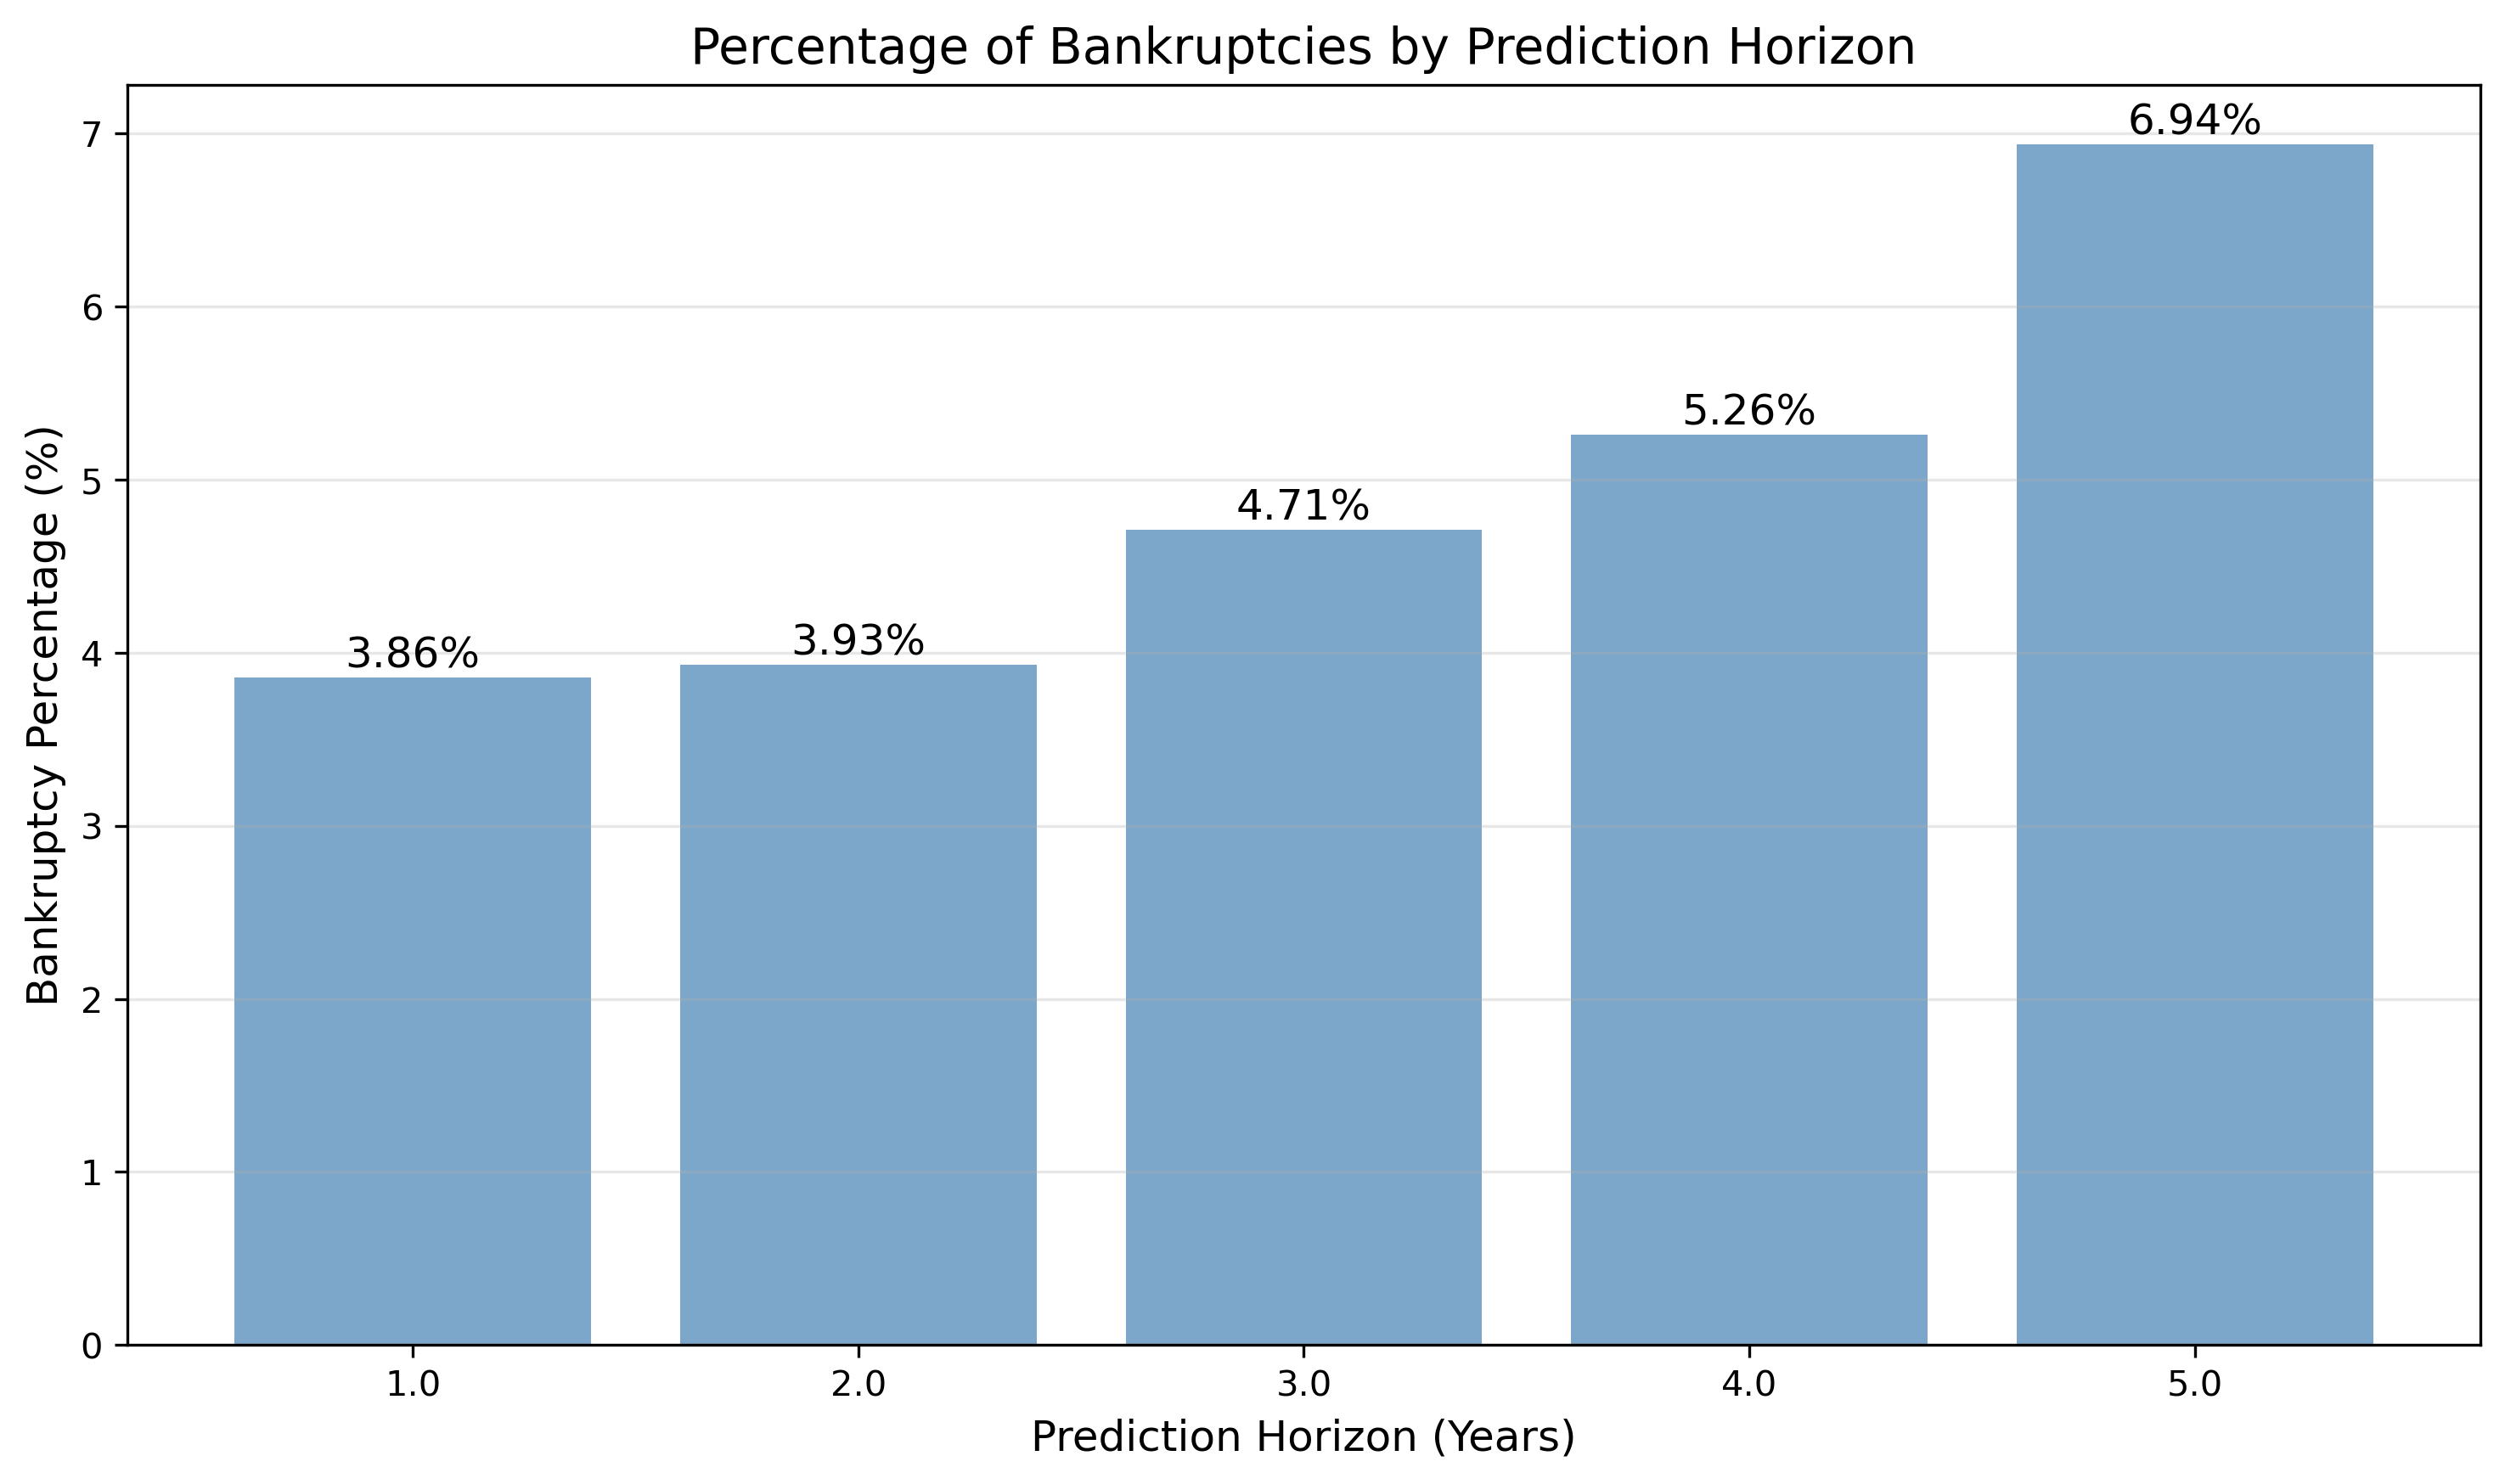
\includegraphics[width=0.8\textwidth]{figures/bankruptcy_by_year.png}
\caption{Percentage of Bankruptcies by Prediction Horizon. The chart shows the distribution of bankruptcy cases across the five prediction timeframes, demonstrating consistent but low bankruptcy rates across all horizons, highlighting the class imbalance challenge.}
\label{fig:bankruptcy_by_year}
\end{figure}

\section{Feature Correlation Analysis}

A comprehensive correlation analysis was conducted to understand the interdependencies among the 64 financial features, providing crucial insights for feature selection and multicollinearity management.

\subsection{High Correlation Identification}

The correlation analysis identified numerous feature pairs exhibiting extremely high correlations (R > 0.95):

\begin{itemize}
    \item \textbf{Perfect Correlations}: Features X7 and X14 showed a correlation of 1.000, indicating complete linear dependence
    \item \textbf{Near-Perfect Correlations}: Multiple feature pairs exhibited correlations exceeding 0.999, suggesting potential redundancy
    \item \textbf{Strong Correlations}: Twenty feature pairs demonstrated correlations above 0.95, warranting careful consideration for feature selection
\end{itemize}

Key high-correlation pairs identified include:
\begin{itemize}
    \item X7 and X14 (r = 1.000)
    \item X4 and X46 (r = 0.999923)
    \item X20 and X56 (r = 0.999878)
    \item X8 and X17 (r = 0.999609)
    \item X19 and X23 (r = 0.999291)
\end{itemize}

\subsection{Hierarchical Clustering for Feature Grouping}

To address the multicollinearity challenge systematically, hierarchical clustering was applied to the correlation matrix:

\textbf{Hierarchical Clustering Algorithm for Feature Selection:}
\begin{enumerate}
\item Compute absolute correlation matrix for all features
\item Calculate pairwise distances using correlation-based metrics
\item Perform hierarchical clustering with average linkage
\item Generate dendrogram visualization
\item Extract optimal cluster configuration (8 clusters selected)
\item Identify largest cluster containing highly correlated features
\end{enumerate}

The clustering analysis revealed:
\begin{itemize}
    \item \textbf{Dominant Cluster}: Cluster 8 contained 17 highly intercorrelated features
    \item \textbf{Feature Redundancy}: Multiple features within the cluster captured similar financial dimensions
    \item \textbf{Selection Strategy}: Representative features were selected from the dominant cluster for model development
\end{itemize}

\begin{figure}[H]
\centering
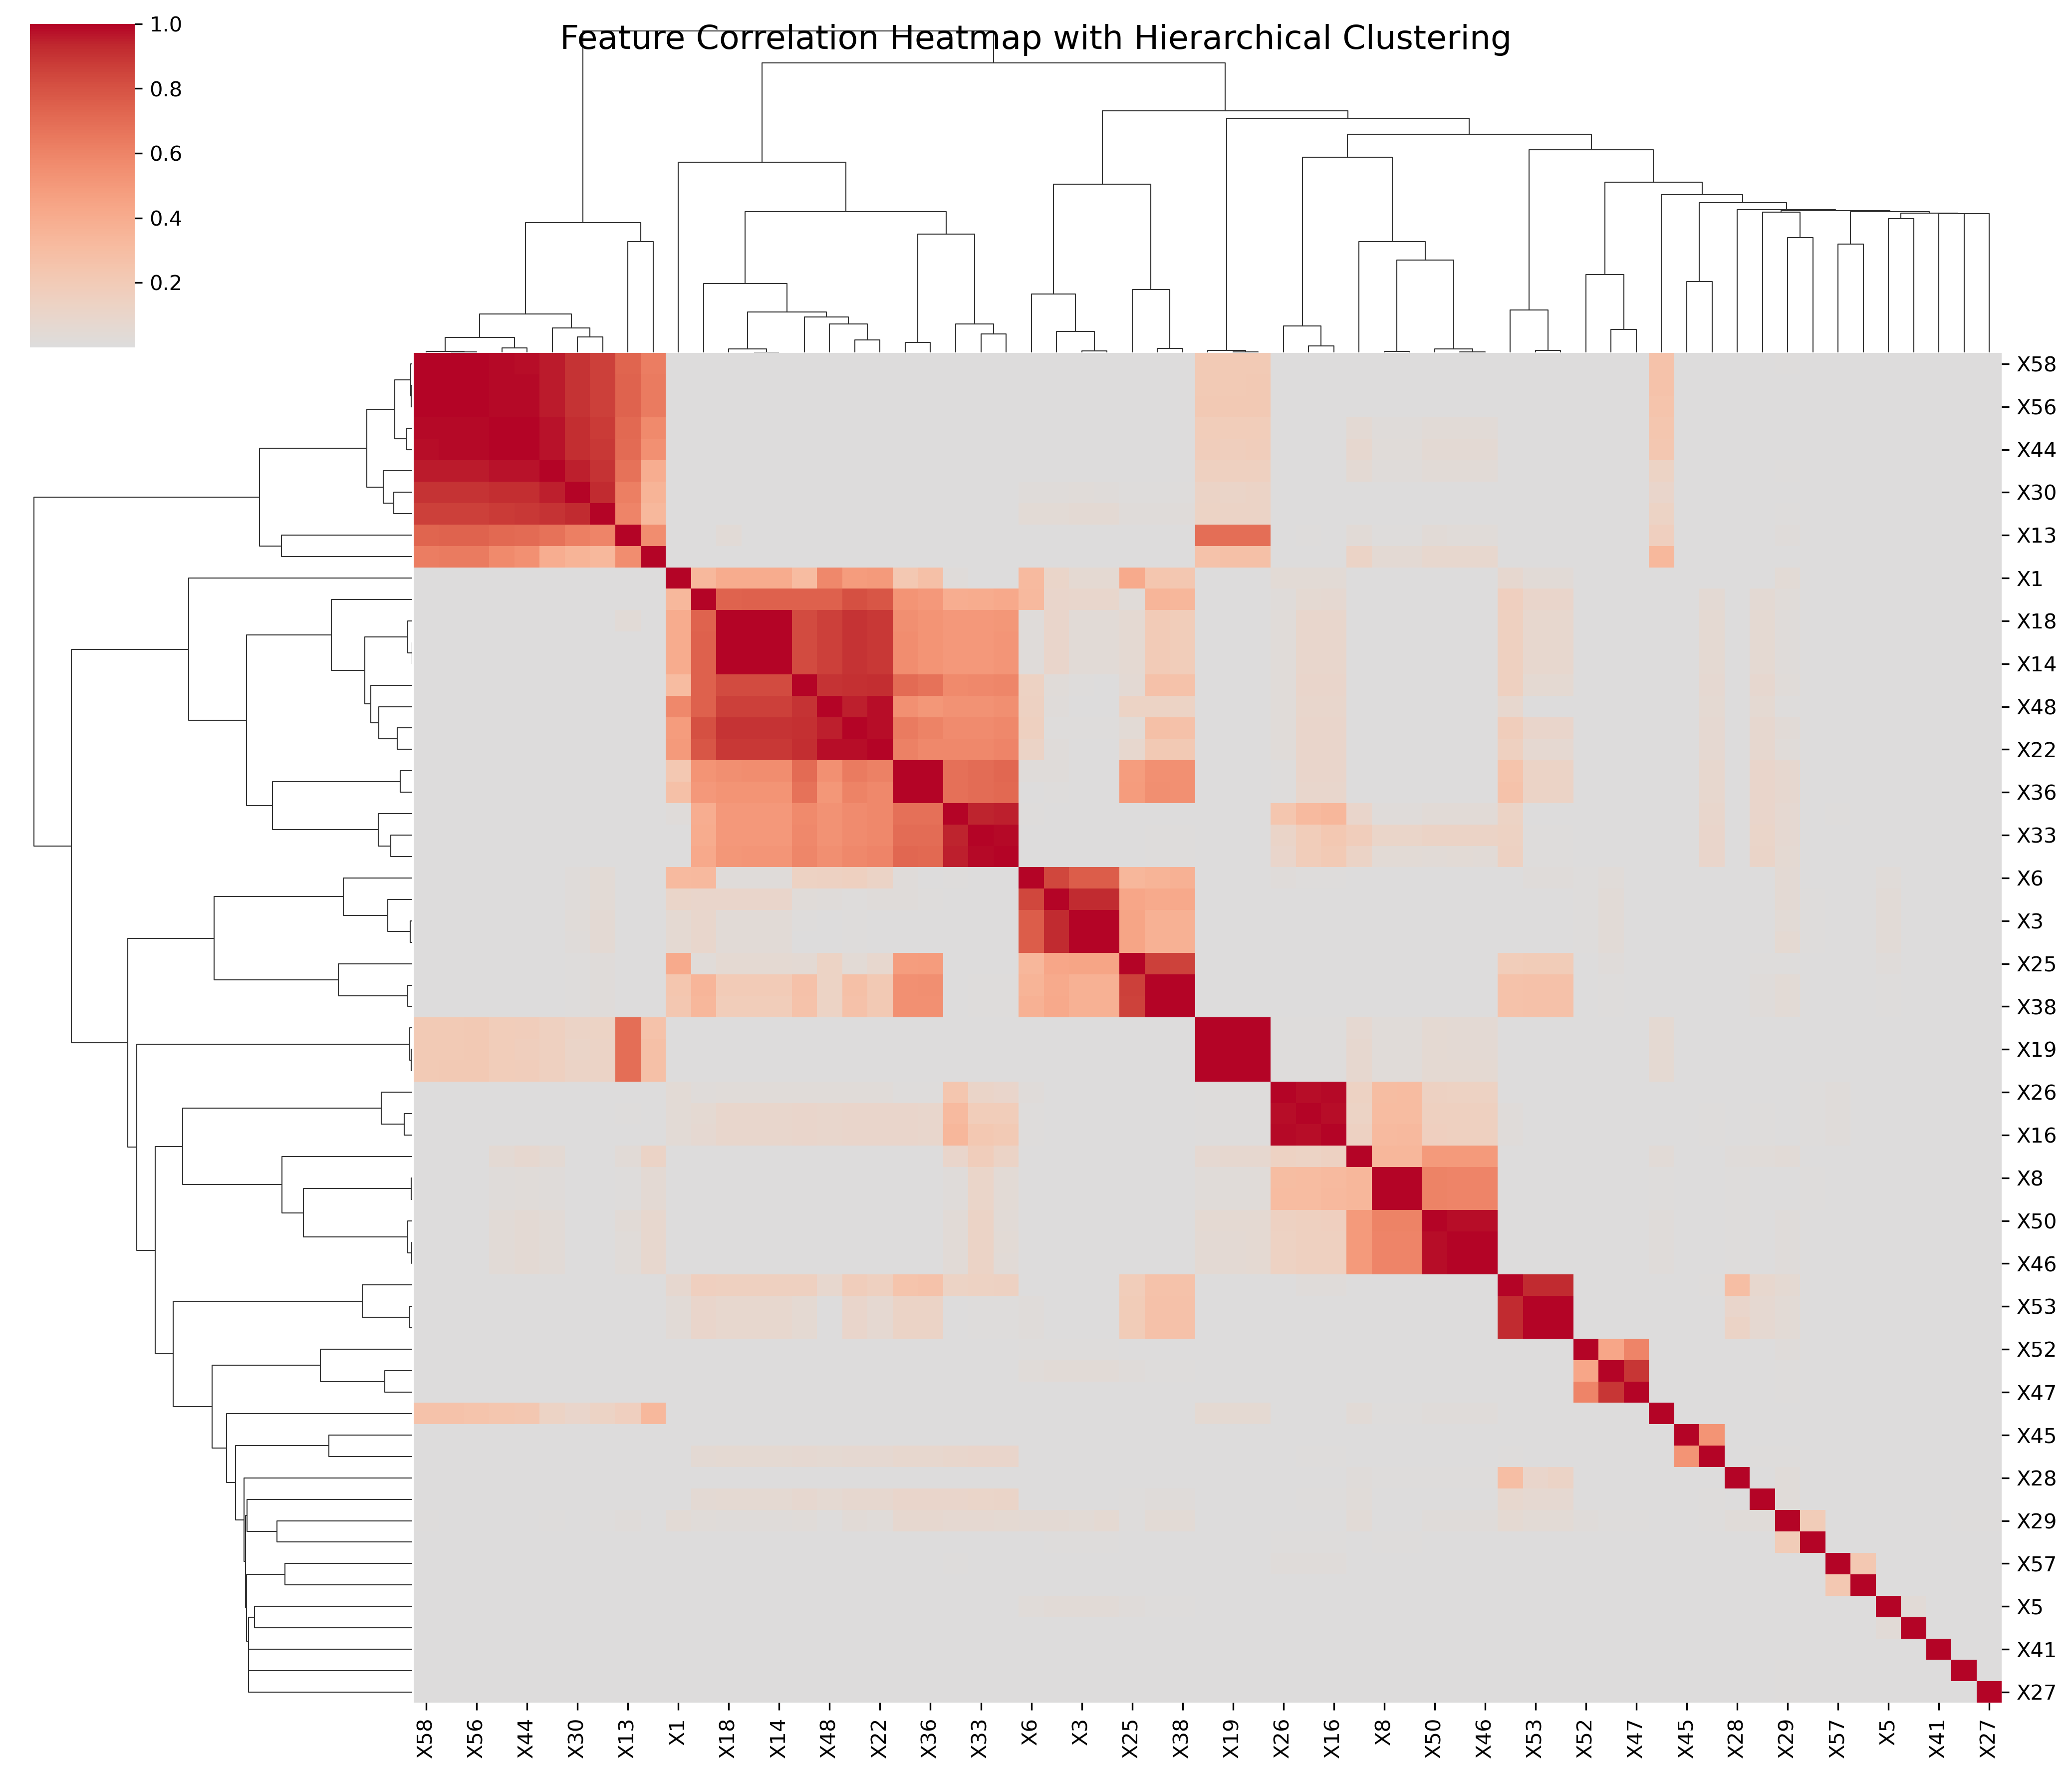
\includegraphics[width=0.95\textwidth]{figures/correlation_clustermap.png}
\caption{Feature Correlation Heatmap with Hierarchical Clustering. The clustermap shows the absolute correlation matrix of all 63 financial features, with hierarchical clustering applied to both rows and columns. Similar features are grouped together, revealing distinct clusters of highly correlated financial ratios.}
\label{fig:correlation_clustermap}
\end{figure}

\section{Feature Selection and Dimensionality Reduction}

Based on the correlation and clustering analyses, a systematic feature selection process was implemented to optimize model performance while minimizing multicollinearity concerns.

\subsection{Selected Feature Set}

From the 17 features in the dominant cluster, a refined subset was selected:

\textbf{Selected Features}: X44, X14, X36, X3, X25, X31, X40, X17, X64, X45, X61, X55, X59, X5, X15

\textbf{Excluded Features}: X51 and X54 were removed due to extreme correlation with retained features.

\subsection{Variance Inflation Factor Analysis}

To validate the feature selection, Variance Inflation Factor (VIF) analysis was conducted on the selected feature set:

\begin{table}[h]
\centering
\caption{Variance Inflation Factors for Selected Features}
\begin{tabular}{|c|c|}
\hline
\textbf{Feature} & \textbf{VIF} \\
\hline
X44 & 1.038 \\
X14 & 1.894 \\
X36 & 2.694 \\
X3 & 1.516 \\
X25 & 2.433 \\
X31 & 1.038 \\
X40 & 1.141 \\
X17 & 1.130 \\
X64 & 1.090 \\
X45 & 1.000 \\
X61 & 1.017 \\
X55 & 1.000 \\
X59 & 1.000 \\
X5 & 1.003 \\
X15 & 1.002 \\
\hline
\end{tabular}
\end{table}

The VIF analysis confirmed the success of the feature selection process:
\begin{itemize}
    \item \textbf{Low VIF Values}: All selected features exhibited VIF values well below the conventional threshold of 5
    \item \textbf{Minimal Multicollinearity}: The highest VIF of 2.694 (X36) indicates acceptable multicollinearity levels
    \item \textbf{Feature Independence}: Most features demonstrated VIF values close to 1, suggesting strong independence
\end{itemize}

\begin{figure}[H]
\centering
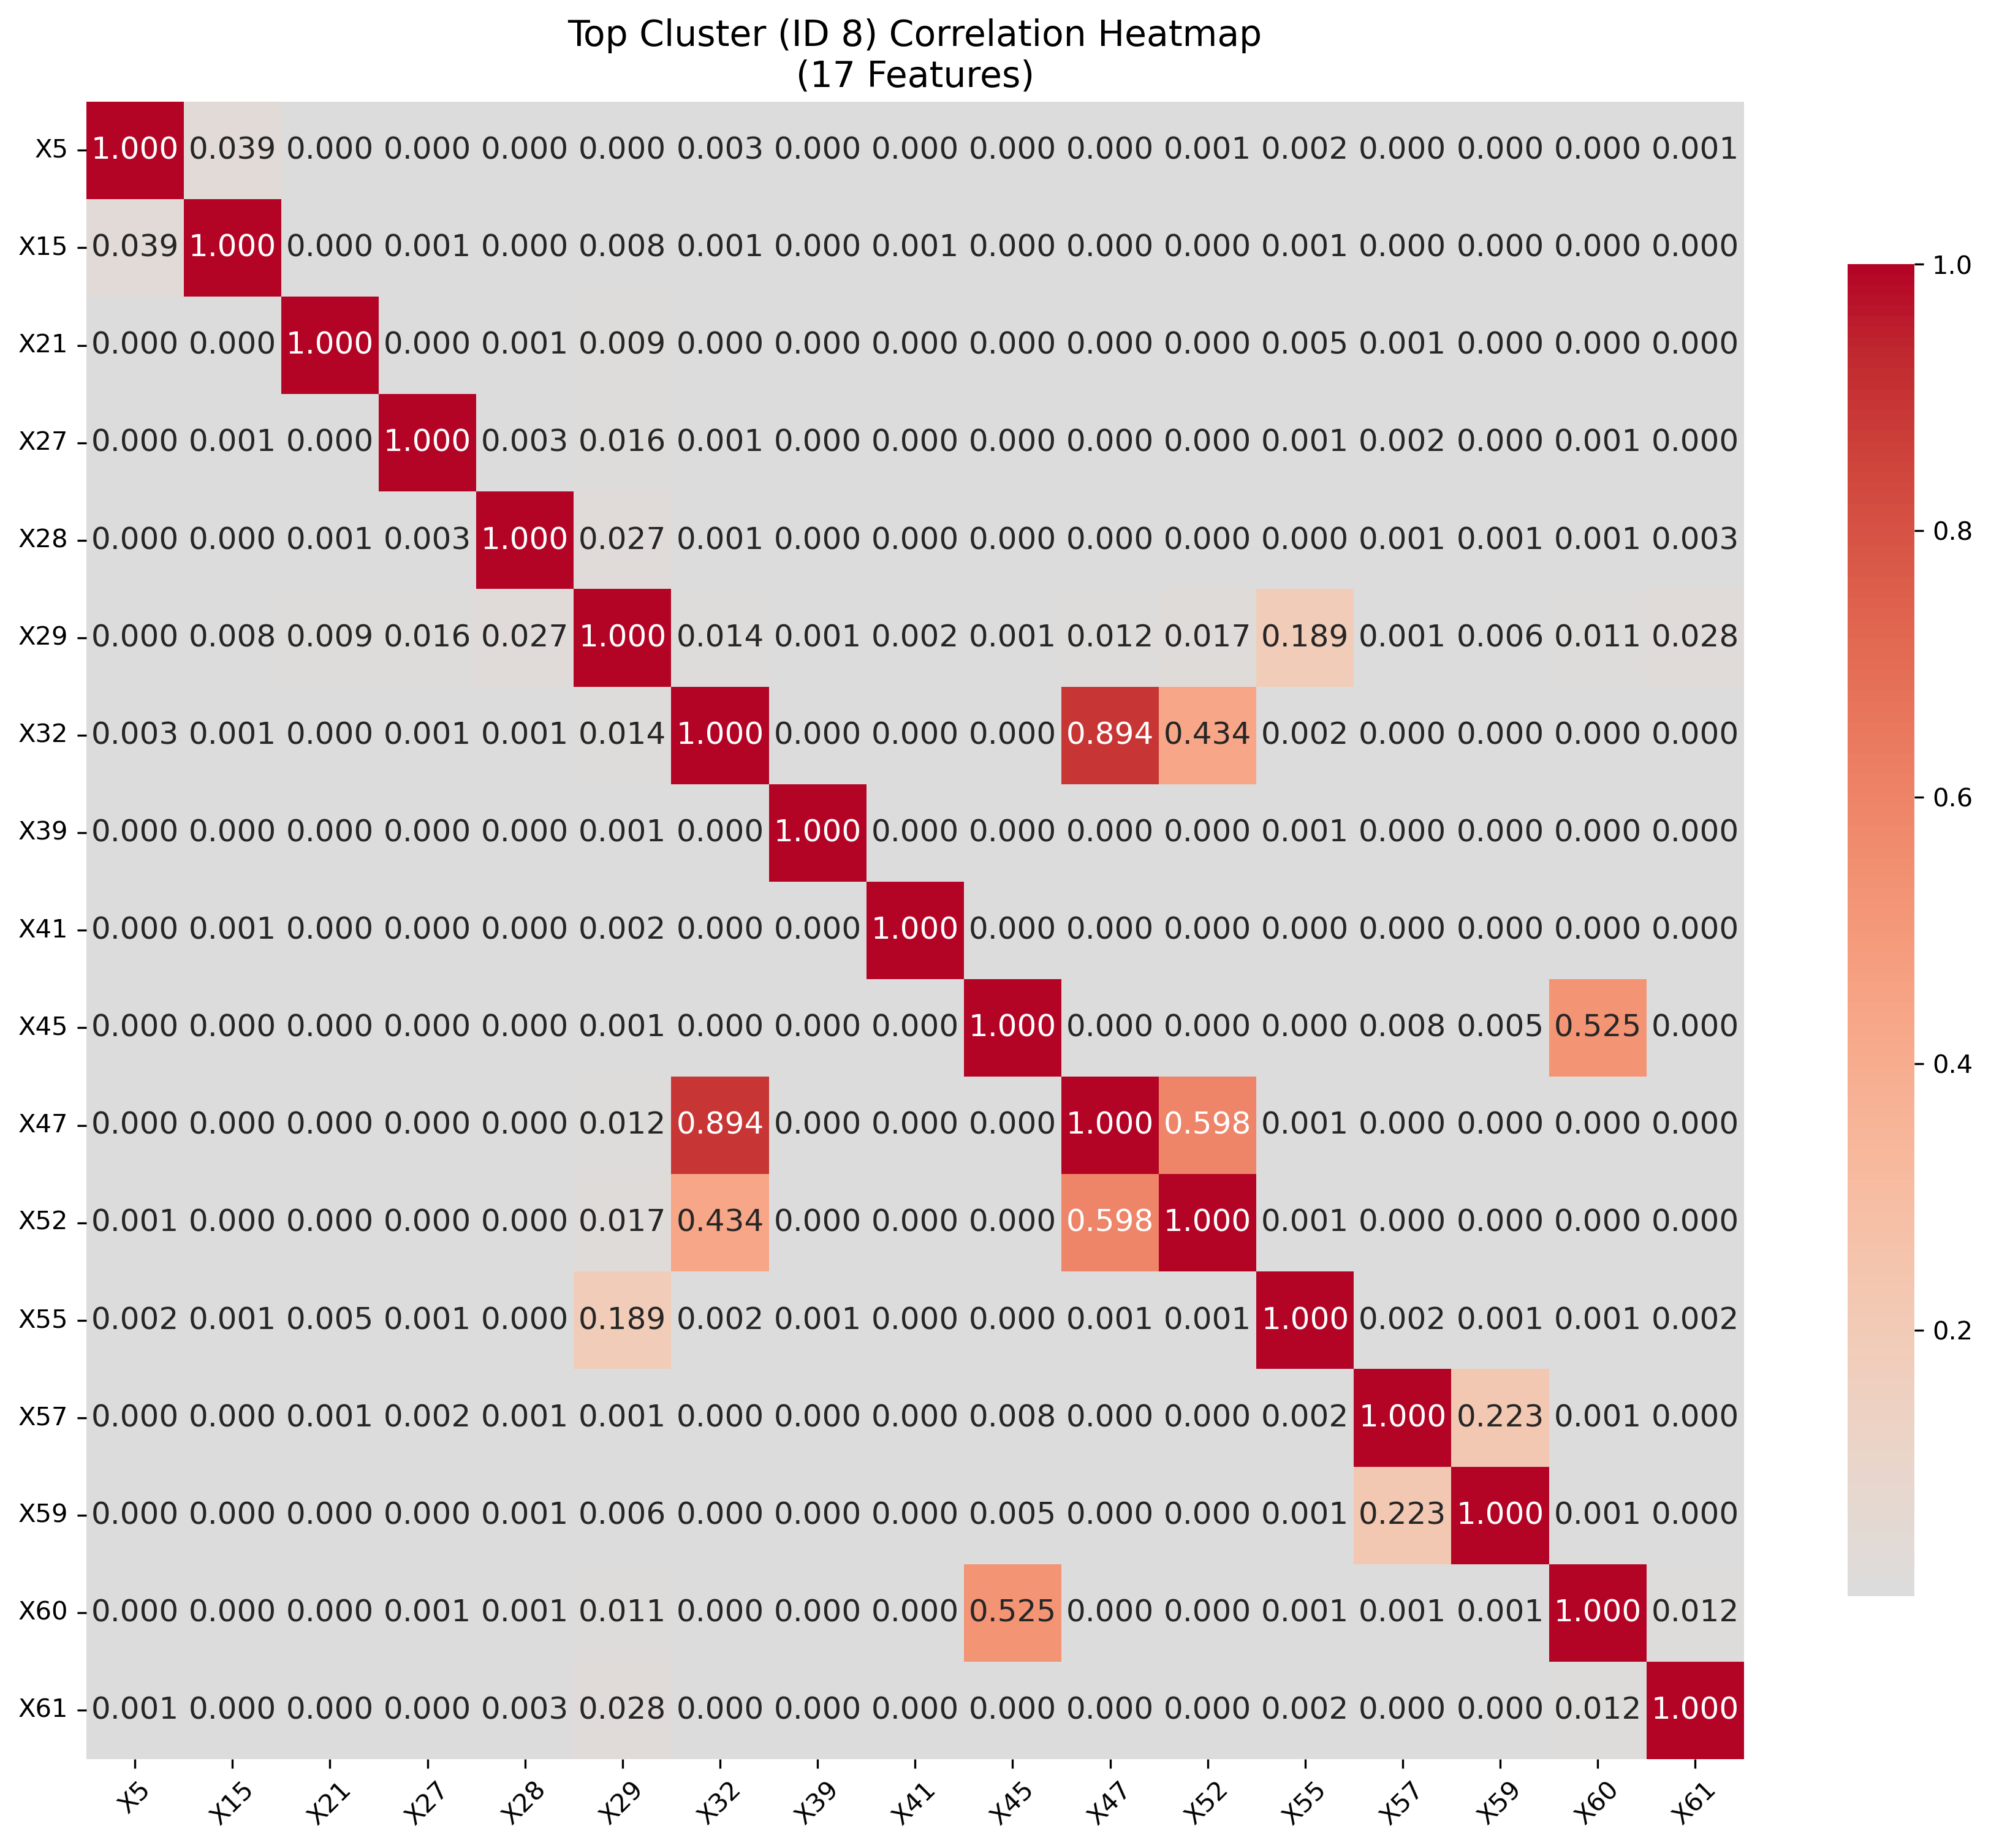
\includegraphics[width=0.9\textwidth]{figures/top_cluster_heatmap.png}
\caption{Top Cluster Correlation Heatmap. This detailed view shows the correlation structure within the dominant cluster (Cluster 8) containing 17 highly intercorrelated features. The annotated correlation coefficients reveal the strength of relationships between features, informing the final selection of 15 representative variables.}
\label{fig:top_cluster_heatmap}
\end{figure}

\section{Data Quality Assessment}

The comprehensive exploratory analysis established a robust foundation for subsequent modeling efforts:

\begin{itemize}
    \item \textbf{Data Completeness}: Post-imputation dataset achieved complete coverage across all analytical features
    \item \textbf{Feature Optimization}: Systematic feature selection reduced dimensionality while preserving predictive information
    \item \textbf{Multicollinearity Management}: VIF analysis confirmed successful mitigation of correlation-induced modeling challenges
    \item \textbf{Temporal Coverage}: Integrated dataset provides comprehensive temporal perspective on bankruptcy patterns
\end{itemize}

These preprocessing and exploration steps ensure that subsequent machine learning models will operate on high-quality, well-structured data optimized for bankruptcy prediction performance. 